\documentclass{ctexart}

%%%% Chinese support
%

%%%% Page geometry
\usepackage[
    a4paper,
    total={210mm,297mm},
    left=20mm,
    right=20mm,
    top=20mm,
    bottom=20mm,
  ]{geometry}            %

%%%% Math
\usepackage{amsmath}     %
\usepackage{siunitx}     % SI unit support

%%%% Caption
\usepackage{caption}
\captionsetup{belowskip=8pt,aboveskip=4pt}


%%%% Graph processing
\usepackage{graphicx}    % graph inclusion

%%%% Table processing
\usepackage{tabularx}
\usepackage{booktabs}    %
\usepackage{csvsimple}   % CSV table processing
\usepackage{multirow}    % multirow in table

%%%% Hyper reference
\usepackage[
    bookmarksnumbered=true,
    colorlinks=true,
    allcolors=blue,
  ]{hyperref}             %

%%%% Bibliography
\usepackage[
    backend=biber,
    style=numeric,
    citestyle=ieee
  ]{biblatex}             %
\addbibresource{compact_debris.bib}

\title{龙卷风风场中块状飞射物的飞行特性}
\author{王勇}

\begin{document}
\maketitle

\begin{abstract}

\end{abstract}

\section{龙卷风风场模型}
龙卷风风场较为复杂,实际工程抗龙卷风计算时,一般对其进行一些简化。
目前工程界主要通过给定龙卷风的特征参数,利用Rankine涡模型确定龙卷风切向速度和压强等流场信息。

\subsection{龙卷风的特征参数}
工程计算采用的龙卷风风场模型,具有如下参数:
(1)最大旋转风速$V_{\mathrm{R}}$;
(2)龙卷风涡的平移速度$V_{\mathrm{T}}$;
(3)最大旋转风速的半径$R$;
(4)气压降$\Delta P$;
(5)气压降速率$\mathrm{d} P/ \mathrm{d} t$。

我国《三十万千瓦压水堆核电厂安全重要土建结构抗龙卷风设计规定》中根据我国国情给出的两组龙卷风设计参数,如表\ref{tab:design_tornado}所示。

\begin{table}[h]
\caption{设计基准龙卷风特性}
\label{tab:design_tornado}
\centering
\begin{tabular*}{\textwidth}{c @{\extracolsep{\fill}} c c c c c c}
    \toprule
    组 & 最大风速 & 旋转风速 & 平移风速 & 最大旋转半径 & 压力降 & 降压时间 \\
    别 & $V (\SI{}{m/s})$ & $V_{\mathrm{R}}  (\SI{}{m/s})$ & $V_{\mathrm{T}}  (\SI{}{m/s})$ & $R (\SI{}{m})$ & $\Delta P (\SI{}{Pa})$ & $t (\SI{}{s})$ \\ \midrule
    A & 107.3 & 84.9 & 22.4 & 45.7 & 8620 & 2.5 \\
    B & 134.1 & 107.3 & 28.8 & 45.7 & 13500 & 1.875 \\ \bottomrule
\end{tabular*}
\end{table}

\subsection{龙卷风的Rankine涡模型}
为了描述龙卷风风场的相关详细信息,工程界采用较多的是由Depperman\cite{Depperman1947}于1947年提出的Rankine涡模型。
Rankine涡模型是满足Navier-Stokes方程的最简单的模型,仅由切向速度控制。
它不考虑径向速度,并假定风速和压强不随高度变化,这在实际情况中是并不存在的。
但研究者最关心的也正是龙卷风的切向速度,因为相比于切向速度,龙卷风的径向速度和竖向速度较小。
其切向速度与离漩涡中心径向位置的关系曲线见图\ref{fig:Rankine}所示:强制涡区域内($r\leq R$)切向速度与半径成正比,而在自由涡区域内($r > R$)成反比。Rankine涡的切向速度表达式为\cite{Commission2007}:

\begin{equation}
\label{eqn:Rankine}
\begin{split}
    V_r &= \frac{r}{R} V_R,  r \leq R \\
    V_r &= \frac{R}{r} V_R,  r > R
\end{split}
\end{equation}
式中:$V_r$是距涡中心为$r$处的切向风速,$V_{\mathrm{R}}$为Rankine涡中的最大切向风速,$R$为最大切向风速对应的旋转半径。

\begin{figure}[h]
\centering
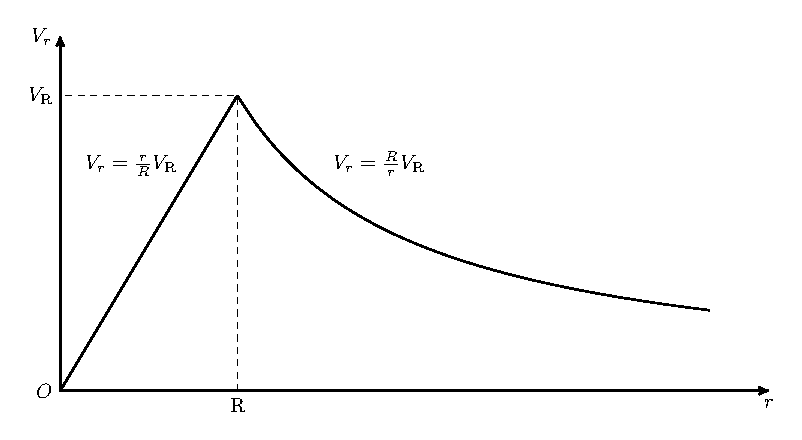
\includegraphics{./fig/Rankine}
\caption{Rankine涡模型中切向速度沿涡半径的变化曲线图}
\label{fig:Rankine}
\end{figure}

\section{块状飞射物的运动方程}
\subsection{问题描述和简化}
考虑龙卷风风场中由静止释放的块状飞射物。龙卷风风场采用Rankine涡模型,不考虑其平移速度。
以龙卷风涡中心为坐标原点,地面为$xOy$坐标面,竖直向上为$z$轴正方向建立空间直角坐标系$O-xyz$,相应建立柱坐标系$O-r\theta z$。
则龙卷风风场切向风速分布由式\eqref{eqn:Rankine}表示。
设飞射物的初始位置为$(r_0,\theta_0,z_0)$。
块状飞射物主要受风阻力的作用(即不考虑其受到的升力和翻转弯矩的影响),由飞射物的相对风速引起的,并沿相对风速的反向。

当不考虑飞射物的竖向速度对相对风速的影响时,块状飞射物的相对风速的量值为$V_r-u_t$,其中$V_r$为龙卷风风场切向风速,$u_t$为飞射物切向速度。
飞射物受到的风阻力$F_D=\frac{1}{2}\rho_a C_D A \left( V_r - u_t \right)^2 $,其中$\rho_a$为空气密度,$C_D$为风阻力系数。

当考虑飞射物的竖向速度对相对风速的影响时,飞射物受到沿相对风速方向的风阻力(相对风速矢量如图\ref{fig:relative_velocity}所示)。相对风速量值为$\sqrt{(V_r-u_t)^2+u_z^2}$,所受的风阻力为$F_D=\frac{1}{2} \rho_a C_D A \left[(V_r-u_t)^2+u_z^2\right] $。

\begin{figure}[h]
\centering
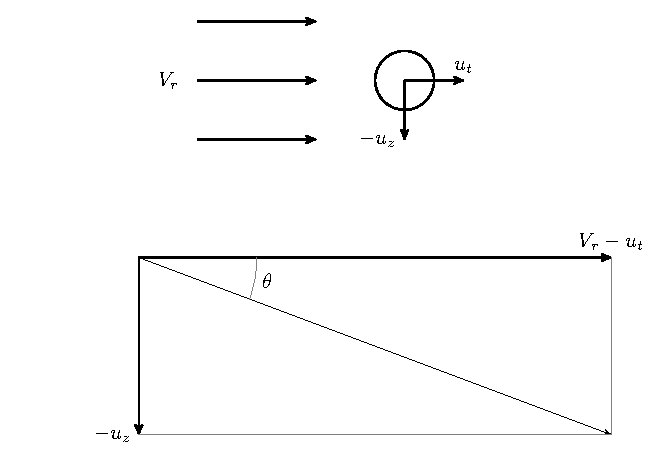
\includegraphics{./fig/relative_velocity}
\caption{运动小球相对风速矢量示意图}
\label{fig:relative_velocity}
\end{figure}

\subsection{不考虑竖向速度对相对风速的影响}
当不考虑竖向速度对相对风速的影响时,飞射物是在切向(水平向)风阻力和竖向重力的联合作用下运动,根据牛顿第二定律列其运动方程如式\eqref{eqn:Newton_no_uz}\eqref{eqn:Newton_no_uz2}:

\begin{equation}
  \label{eqn:Newton_no_uz}
      m\frac{\mathrm{d}^2 \left(r_0 \theta \right)}{\mathrm{d} t^2} = m\frac{\mathrm{d} u_t}{\mathrm{d} t} = \frac{1}{2} \rho_a C_D A \left(V_r-u_t\right)^2
\end{equation}

\begin{equation}
  \label{eqn:Newton_no_uz2}
  m\frac{\mathrm{d}^2 z}{\mathrm{d} t^2} = m\frac{\mathrm{d} u_z}{\mathrm{d} t } = -mg
\end{equation}
定义参数
\begin{equation}
k=\frac{\rho_a C_D}{2 \rho_m \ell}
\end{equation}
其中$\rho_m$为飞射物的密度,$\ell$为飞射物的参考长度,即飞射物体积与迎风面积的比值。
则块状飞射物的运动方程可简化为式\eqref{eqn:Newton_no_uz3}\eqref{eqn:Newton_no_uz4}:

\begin{equation}
  \label{eqn:Newton_no_uz3}
      \frac{\mathrm{d}^2 \left(r_0 \theta\right)}{\mathrm{d} t^2} = \frac{\mathrm{d} u_t}{\mathrm{d} t} = k \left(V_r-u_t\right)^2
\end{equation}

\begin{equation}
\label{eqn:Newton_no_uz4}
\frac{\mathrm{d}^2 z}{\mathrm{d} t^2} = \frac{\mathrm{d} u_z}{\mathrm{d} t } = -g
\end{equation}
 

式\eqref{eqn:Newton_no_uz3}为非耦联的方程,因此可以通过分离变量法直接求其解析解:
对飞射物切向的运动方程进行分离变量和积分,积分结果为
\begin{equation}
t=\int \frac{1}{k \left(V_r-u_t\right)^2} \mathrm{d} u_t =\frac{u_t}{k\left(V_r-u_t\right) V_r}.
\end{equation}
则不考虑物体竖向运动对风作用力的影响时块状飞射物的切向运动速度为:

\begin{equation}
  \label{eqn:velocity_no_uz}
    u_t=\frac{kV_r^2 t}{1+k V_r t}
\end{equation}
式\eqref{eqn:velocity_no_uz}对于时间$t$积分可得:
\begin{equation}
  \label{eqn:displacement_no_uz}
    \theta=\theta_0+\frac{V_r}{r_0} \left[t-\frac{1}{k V_r} \ln \left(1+kV_r t\right)\right]
\end{equation}

上述的推导仅考虑水平风阻力的作用,则飞射物在竖向仅受重力的作用,则物体竖向的速度和位移为:
\begin{equation}
u_z=-gt
\end{equation}
\begin{equation}
z=z_0-\frac{1}{2}gt^2
\end{equation}
\subsection{考虑竖向风速对相对风速的影响}
当考虑物体竖向运动对风作用力的影响时,飞射物受到沿相对风速方向的风阻力以及竖向重力作用。
把风阻力分解成切向和竖向两部分:$F_{Dr} = F_D \cos \beta$, $F_{Dz} = F_D \sin \beta$。
其中$\beta$为相对风速与切向风速的夹角。由图\ref{fig:relative_velocity}可得:
\begin{equation}
\cos \beta=\frac{V_r-u_t}{\sqrt{(V_r-u_t)^2+u_z^2}}
\end{equation}
\begin{equation}
\sin \beta=\frac{-u_z}{\sqrt{(V_r-u_t)^2+u_z^2}}
\end{equation}
则飞射物在竖向所受到的作用力为:
\begin{equation}
F_z = F_D \sin \beta - mg
\end{equation}

则考虑物体竖向运动对风作用力的影响时,块状飞射物的运动方程为\cite{Holmes2004}:
\begin{equation}
\label{eqn:Newton_uz}
\begin{split}
\frac{\mathrm{d}^2 (r_0 \theta)}{\mathrm{d} t^2} = \frac{\mathrm{d} u_t}{\mathrm{d} t}& = \frac{\rho_a C_D (V_r - u_t)\sqrt{\left(V_r-u_t\right)^2+u_z^2}}{2\rho_m \ell} \\
 & = k\left(V_r-u_t\right)\sqrt{\left(V_r-u_t\right)^2+u_z^2}
\end{split}
\end{equation}

\begin{equation}
\label{eqn:Newton_uz2}
\begin{split}
  \frac{\mathrm{d}^2 z}{\mathrm{d} t^2} = \frac{\mathrm{d}u_z}{\mathrm{d} t}&=  \frac{\rho_a C_D ( - u_z)\sqrt{\left(V_r-u_t\right)^2+u_z^2}}{2\rho_m \ell} -g \\
   & = k\left(-u_z\right)\sqrt{\left(V_r-u_t\right)^2+u_z^2}-g
\end{split}
\end{equation}

由于$u_z$在数值上是负的(块状飞射物的竖向运动速度是向下的),因此由重力产生的竖向加速度与由风作用力产生的竖向加速度方向是相反的。

式\eqref{eqn:Newton_uz}和\eqref{eqn:Newton_uz2}是耦联的方程,不能直接求其解析解,但可以用小时间步法\cite{Baker2004}求其水平和竖向的加速度、速度和位移。


\printbibliography
\end{document}
